\clearpage

\def\chaptertitle{Experimental Setup}

\lhead{\emph{\chaptertitle}}

\chapter{\chaptertitle}
\label{ch:experimental-setup}

In this chapter, we will first discuss the underlying hardware and assumptions used in creating the experiments in section \ref{sec:ch4-hardware-assumptions}. Section \ref{sec:ch4-microservice-overview} will then describe the microservice application used to test the algorithm, along with the method used to generate data. Finally, we will discuss the proposed algorithm itself, and how each subsection of the autoscaler interacts with Kubernetes.

\section{Assumptions and Underlying Hardware}
\label{sec:ch4-hardware-assumptions}

For the hardware setup, servers in the Melbourne Research Cloud \footnote{\url{https://docs.cloud.unimelb.edu.au/}} were leveraged to deploy microservices on. The set up consisted of 6 servers, using a total of 16 CPU cores and 32GB of memory. These servers were separated into a cloud and edge layer. The servers on the cloud layer have a significantly higher amount of CPU cores and memory assigned compared to the servers in the edge layer, to simulate the scarcity of resources in the edge layer. Furthermore, a simulated latency was added between inter-layer server communication to mimic the perceived distance between edge nodes and large data-centres.\par

Kubernetes is used as the container orchestration technology behind the experimental microservice setup. The control plane is deployed on the cloud layer, while the data plane is on the edge layer. Furthermore, several assumptions were made before proceeding with the experimentation:

\begin{itemize}
    \item The only autoscaling performed would be horizontal pod autoscaling. Vertical and cluster autoscaling were out of scope of the project.
    \item The pods on which autoscaling are not applied will have the maximum possible resource allocation to remove the chances of bottleneck.
    \item At no point in the experiment would a node be taken down, or new node be added.
    \item The autoscaler assumes that every node in the edge layer is an equally likely candidate for scheduling pods on.
\end{itemize}

\section{Microservice Overview}
\label{sec:ch4-microservice-overview}

DeathStarBench \footnote{\url{https://github.com/delimitrou/DeathStarBench/tree/master/socialNetwork}}, a social media microservice developed by Y. Gan et al. \cite{gan2019open} is deployed on Kubernetes. The application mimics a large-scale social network application and supports creating user posts on their timeline, reading other user timelines, and receiving follower recommendations. Figure \ref{fig:social} shows the architecture of the micro-service.\par

The architecture is divided into three layers. The frontend consists of the load balancer and web server deployments. The logic backend layer consists of deployments used to send and receive the APIs required for creating user posts, reading timelines, authenticating users, search features, and generating recommendations. Finally, the storage layer comprises of Redis and MongoDB deployments for storing the timeline and user data.\par

Users can sign in to the application website by connecting to the user interface deployment, which can be assigned a DNS address. For experimental purposes, we simply use the Kubernetes node IP address and the social media service port. For example, an API request for reading user timelines will look as follows:\par

http://<node-IP>:<social-media-port>/wrk2-api/user-timeline/read

\begin{figure}[htb]
    \centering
    \caption{DeathStarBench Social-Network Architecture, courtesy Y. Gan et al. \cite{gan2019open}}
    \label{fig:social}
    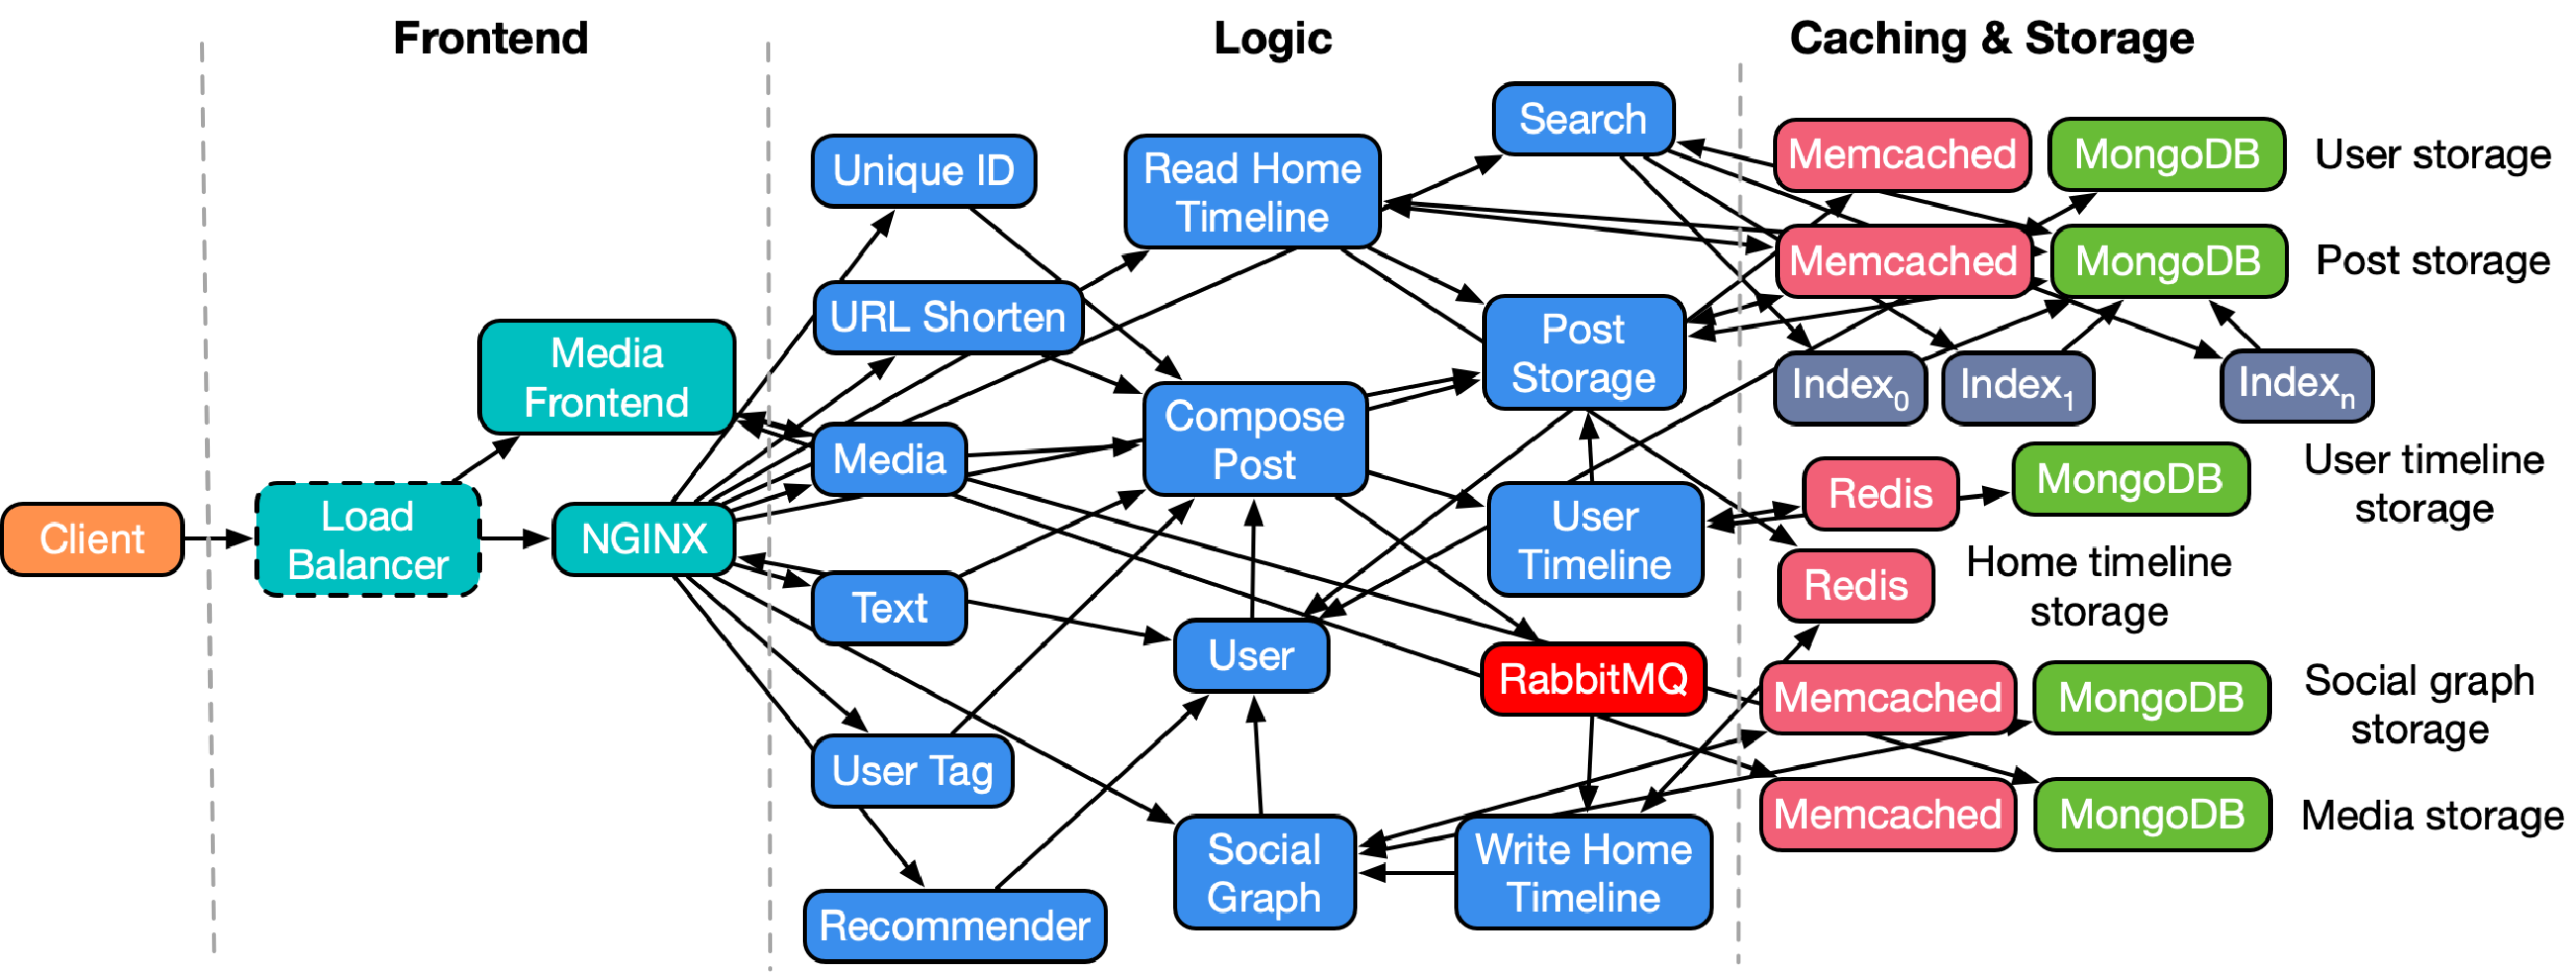
\includegraphics[width=1.0\linewidth]{Figures/Social-Network-Architecture.pdf}
\end{figure}

\section{Data Generation}
\label{sec:data-generation}

The social media deployment also comes with an HTTP workload generator, which
is leveraged to create a realistic simulation of a typical day of workload for the microservice application. The generator, known as ``wrk2'', is an open-loop load generator. HTTP requests are sent out according to the user configuration, regardless of whether or not the responses of the previous requests have been received. This avoids issues such as queuing delays in the server. The workload generator supports a variety of load generation use-cases, as well as different APIs. For example, a POST request a total load generation of 10 requests per second using 2 threads, with 5 open HTTP connections, and for a duration of 30 seconds looks like:\par

wrk2 -t2 -c5 -d30s -R10 http://<node-IP>:<social-media-port>/wrk2-api/post/compose\par

A typical IoT application in the edge has a semi-predictable workload pattern. In this experiment, it is assumed that the workload peaks in the morning and evening, while seeing moderate usage during the afternoon. The workload is lowest at night. The workload simulator was modified to introduce an element of randomness to mimic realistic weekly workloads, which can vary on occasions such as weekends and public holidays.\par

To achieve this, an IoT workload algorithm was created for leveraging the wrk2 generator to achieve this time-series. This is explained in algorithm \ref{alg:work-gen}. A constant workload is set for night time, while different workloads for different day time hours are set. The algorithm also contains a small random ``offset'' variable to depict the randomness inherent in the workload. This workload is then executed using the wrk2 generator to apply the HTTP load on the microservice.

%TC:ignore
\begin{algorithm}
    \caption{IoT workload generation algorithm}
    \label{alg:work-gen}
    \begin{algorithmic}
        \State $offset \gets \alpha$
        \State $night\_workload \gets \omega$
        \State $day\_workload \gets [ \delta_1, \delta_2, ... , \delta_{18}]$
        \While{True}
            \For {i $\leftarrow$ 0 ... 6}
                \State $result \gets generate(night\_workload + \mathcal{U}(-offset,offset)$
            \EndFor
            \For {i $\leftarrow$ 0 ... 18}
                \State $result \gets generate(day\_workload[i] + \mathcal{U}(-offset,offset)$
            \EndFor
        \EndWhile
    \end{algorithmic}
\end{algorithm}
%TC:endignore

\section{Hybrid Autoscaler Architecture}
\label{ref:hybrid-auto-arch}

\suhrid{Elaborate on this section. Put the detailed hybrid architecture diagram here and explain it before going through the individual sections. Use the text in Euro-Par paper}

In this section, the overall architecture of our proposed hybrid autoscaler will be discussed. First, a brief background of how the social media application is connected to Kubernetes, so that it can send custom metrics such as application CPU usage and latency. Then we will discuss these custom metrics further, and how they are integrated for use in the horizontal pod autoscaler.\par

With this background, we proceed with the discussion of the reactive subcomponent of the hybrid autoscaler, discussing its architecture and overall role within the algorithm. We then discuss the proactive autoscaler. This includes the components which are used to train the time-series analyzer, the choice of algorithm, and the overall goals of the forecaster. Finally, the autoscaler daemon, which controls the reactive and proactive subcomponents, as well as tunes the proactive autoscaler, will be briefly discussed.\par

\subsection{Social Media Metrics Export To Kubernetes}
\label{subsec:metrics-export}

The social media application comes bundled with Jaeger \footnote{\url{https://www.jaegertracing.io/}} deployment. Jaeger is an open-source distributed tracing platform, capable of tracking several application metrics. One such metric is the details of API latency for the application. The latency information is extremely detailed, and is broken down per each deployment in the social media architecture as defined by Figure \ref{fig:social}.\par

Before this information can be useful in the autoscaling solution, it must be imported to Kubernetes in a readable format. This was achieved through the use of a deployment called Prometheus. Prometheus \footnote{\url{https://prometheus.io/docs/introduction/overview/}} is an open-source deployment used for monitoring applications. Prometheus consists of a multi-dimensional data model for storing time-series data through key/value pairs, a custom built querying language known as PromQL, which is used to leverage and search through this data model, and a graphing and dashboard user interface to aid in visualization.\par

To facilitate the export of Jaeger metrics to Prometheus, a custom deployment was created which scrapes these metrics at a given time interval, and pushes it to Prometheus. The ``Jaeger-Scraper'' deployment was a JavaScript express server using the open-source prometheus-client library, and the server code was as follows:

%TC:ignore
\begin{lstlisting}[
  caption={Jaeger-Scraper server},
  captionpos=t,
  label={lst:jaeger-scraper},
  float=ht
]
const avg_counter = new Gauge({
        name: 'wrk2_avg_api_latency',
        help: 'Jaeger average post API latency (ms)'
});

get('/metrics', async (req, res) => {
    let url = process.env.JAEGER_URL;
    const data = await axios.get(url);
    let avg_duration = 0;

    let durations = data.map(api => {
        let duration = api.spans.find(
            span => span.references.length === 0
        );
        return duration;
    });

    avg_duration = durations.reduce( (a,b) => a+b ) / durations.length;
    avg_counter.set(avg_duration);

    res.set('Content-Type', avg_counter);
});
\end{lstlisting}
%TC:endignore

Once this server is deployed on the Kubernetes cloud layer, a service-monitor for Prometheus is written, which tells Prometheus to invoke the GET API this server exposes at a set interval of time. For this thesis, this interval was set at 15 seconds.

%TC:ignore
\begin{lstlisting}[
  caption={Jaeger-Scraper service monitor},
  captionpos=t,
  label={lst:jaeger-scraper svc-monitor},
  float=ht
]
apiVersion: monitoring.coreos.com/v1
kind: ServiceMonitor
metadata:
  labels:
    app: jaeger-scraper
  name: jaeger-scraper-svc-monitor
spec:
  endpoints:
  - interval: 15s
    port: http
  selector:
    matchLabels:
      app: jaeger-scraper
\end{lstlisting}
%TC:endignore

Listing \ref{lst:jaeger-scraper-metric} below shows an example of how the metrics are displayed. With the latency metrics now present in Prometheus, the next step to importing these metrics to the custom metrics server was deployed.\par

%TC:ignore
\begin{lstlisting}[
  caption={Jaeger-Scraper metrics collector},
  captionpos=t,
  label={lst:jaeger-scraper-metric},
  float=ht
]
ubuntu@k8s:~$ curl $(kubectl get service jaeger-scraper \
--template '{{.spec.clusterIP}}'):8081/metrics
# HELP wrk2_avg_api_latency Jaeger average post API latency (ms)
# TYPE wrk2_avg_api_latency gauge
wrk2_avg_api_latency 0
\end{lstlisting}
%TC:endignore

By default, Kubernetes autoscaling can scale resources based on CPU and memory utilization. However, for more complex use-cases, more metrics need to be taken into account to make such decisions. To aid in this process, the Prometheus Adapter \footnote{\url{https://github.com/kubernetes-sigs/prometheus-adapter}} was created to leverage the metrics collected and stored by the Prometheus deployment, and feed them to Kubernetes. These metrics are exposed via an API service and are consumed by the hybrid autoscaler for decision making.\par

The prometheus adapter requires a configuration map (ConfigMap) to translate Prometheus metrics to Kubernetes custom metrics. The adapter does so in four steps.

\begin{itemize}
    \item Discovery - The adapter discovers the metrics available in Prometheus
    \item Association - Figure out the association between each metric and Kubernetes resource
    \item Naming - Assigns a name to these resources through which the custom metrics API can expose them
    \item Querying - Queries the Prometheus deployment to get the actual metric numbers
\end{itemize}

The hybrid autoscaler requires the default CPU metric, as well as the custom latency metric. Thus we define these this additional metric for configuring in Kubernetes. Listing \ref{lst:prometheus-adapter-configmap} shows the discovery, association, naming, and querying steps to do so.

%TC:ignore
\begin{lstlisting}[
  caption={Prometheus adapter configmap},
  captionpos=t,
  label={lst:prometheus-adapter-configmap},
  float=ht
]
apiVersion: v1
kind: ConfigMap
metadata:
  name: custom-metrics-prometheus-adapter
data:
  config.yaml: |
    rules:
    - metricsQuery: <<.Series>>
      name:
        as: ${1}_per_minute
        matches: ^(.*)
      resources:
        template: <<.Resource>>
      seriesQuery: wrk2_avg_api_latency{namespace!=""}
\end{lstlisting}
%TC:endignore

Now, the Kubernetes custom metrics API exposes the following additional APIs in listing \ref{lst:custom-metrics-example}

%TC:ignore
\begin{lstlisting}[
  caption={Custom metrics API example},
  captionpos=t,
  label={lst:custom-metrics-example},
  float=ht
]
ubuntu@k8s:~$ kubectl get --raw /apis/custom.metrics.k8s.io/v1beta1 | jq .
{
  "groupVersion": "custom.metrics.k8s.io/v1beta1",
  "resources": [
    {
      "name": "services/wrk2_avg_api_latency_per_minute",
      ...
    },
    {
      "name": "pods/wrk2_avg_api_latency_per_minute",
      ...
    },
    {
      "name": "namespaces/wrk2_avg_api_latency_per_minute",
      ...
    }
  ]
}

ubuntu@k8s:~$ kubectl get --raw \
/apis/custom.metrics.k8s.io/v1beta1\
/namespaces/default/services/*/wrk2_avg_api_latency_per_minute \
| jq .
{
  "kind": "MetricValueList",
  "apiVersion": "custom.metrics.k8s.io/v1beta1",
  "items": [
    {
      "describedObject": {
        "kind": "Service",
        ...
      },
      "metricName": "wrk2_avg_api_latency_per_minute",
      "value": "0"
    }
  ]
}


\end{lstlisting}
%TC:endignore

\subsection{Reactive Autoscaler}
\label{subsec:reactive-auto-subsection}

\suhrid{TODO: Add the forecast cpu configmap to the listings later, it is mentioned here in a comment.}
\begin{comment}
%TC:ignore
\begin{lstlisting}[
  caption={Prometheus adapter configmap},
  captionpos=t,
  label={lst:prometheus-adapter-configmap},
  float=ht
]
- metricsQuery: <<.Series>>
  name:
    as: ${1}_per_minute
    matches: ^(.*)
  resources:
    template: <<.Resource>>
  seriesQuery: forecasted_cpu{namespace!=""}
- metricsQuery: <<.Series>>
  name:
    as: ${1}
    matches: ^(.*)
  resources:
    template: <<.Resource>>
  seriesQuery: forecasted_cpu_avg{service!=""}
\end{lstlisting}
%TC:endignore
\end{comment}